\chapter{Results and Analysis}
\label{sec:results}

\section{Dataset Analysis: LIGHT}
\label{sec:analysis-light}

As described in section \ref{sec:method-features} on page \pageref{sec:method-features}, a visualization of a LIGHT subsample from January 1st, 2020 was developed and is shown in figure \ref{fig:overview-light}. The visualization features a five-dimensional graph and depicts the geographical distribution of lightning strikes, with longitude and latitude represented by the x and y axes respectively. The z-axis indicates the number of lightning strikes that occurred at each location, while the color of the dots represents the time of occurrence.

From the graph, we can observe that lightning strikes tend to occur in sequences with close temporal proximity. This suggests that binning or grouping of the lightning strikes may prove beneficial.

\begin{figure}[H]
	\centering
	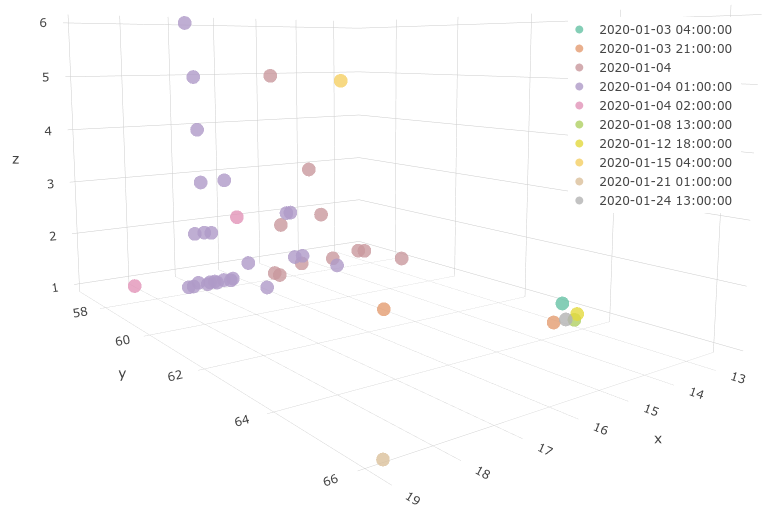
\includegraphics[width=\linewidth, keepaspectratio]{figures/light-graph}
	\caption{Visualization of the LIGHT dataset during January 1st, 2020.}
	\label{fig:overview-light}
\end{figure}

\section{Dataset Analysis: MESAN}

\subsection{Exploratory Analysis}

Upon manual inspection, it is evident that the MESAN dataset contains numerous observations with missing values. Some variables, such as \texttt{24-hour precipitation} and \texttt{12-hour snow} have all values missing except for at the specific intervals. Additionally, the parameters \texttt{minimum temperature} and \texttt{maximum temperature} are completely missing, likely due to a mistake in SMHI's documentation. All empty or time-dependent fields were dropped from the dataset as they do not provide any additional information to the models. 

Furthermore, it is assumed that certain fields are highly correlated, such as derived and related measurements. To verify this assumption, a covariance matrix was utilized (see section \ref{sec:analysis-mesan-correlation}).

\subsection{Correlation Analysis}
\label{sec:analysis-mesan-correlation}

The covariance matrix for the MESAN dataset provides information about the correlation between different parameters. Figure \ref{fig:mesan-covariance-matrix-before-analysis} shows the correlation matrix for a subset of the MESAN data, which consists of 458,328 observations. The \texttt{Snowfall} parameter was excluded from the analysis as it only contained zeroes. 

\begin{figure}[H]
	\centering
	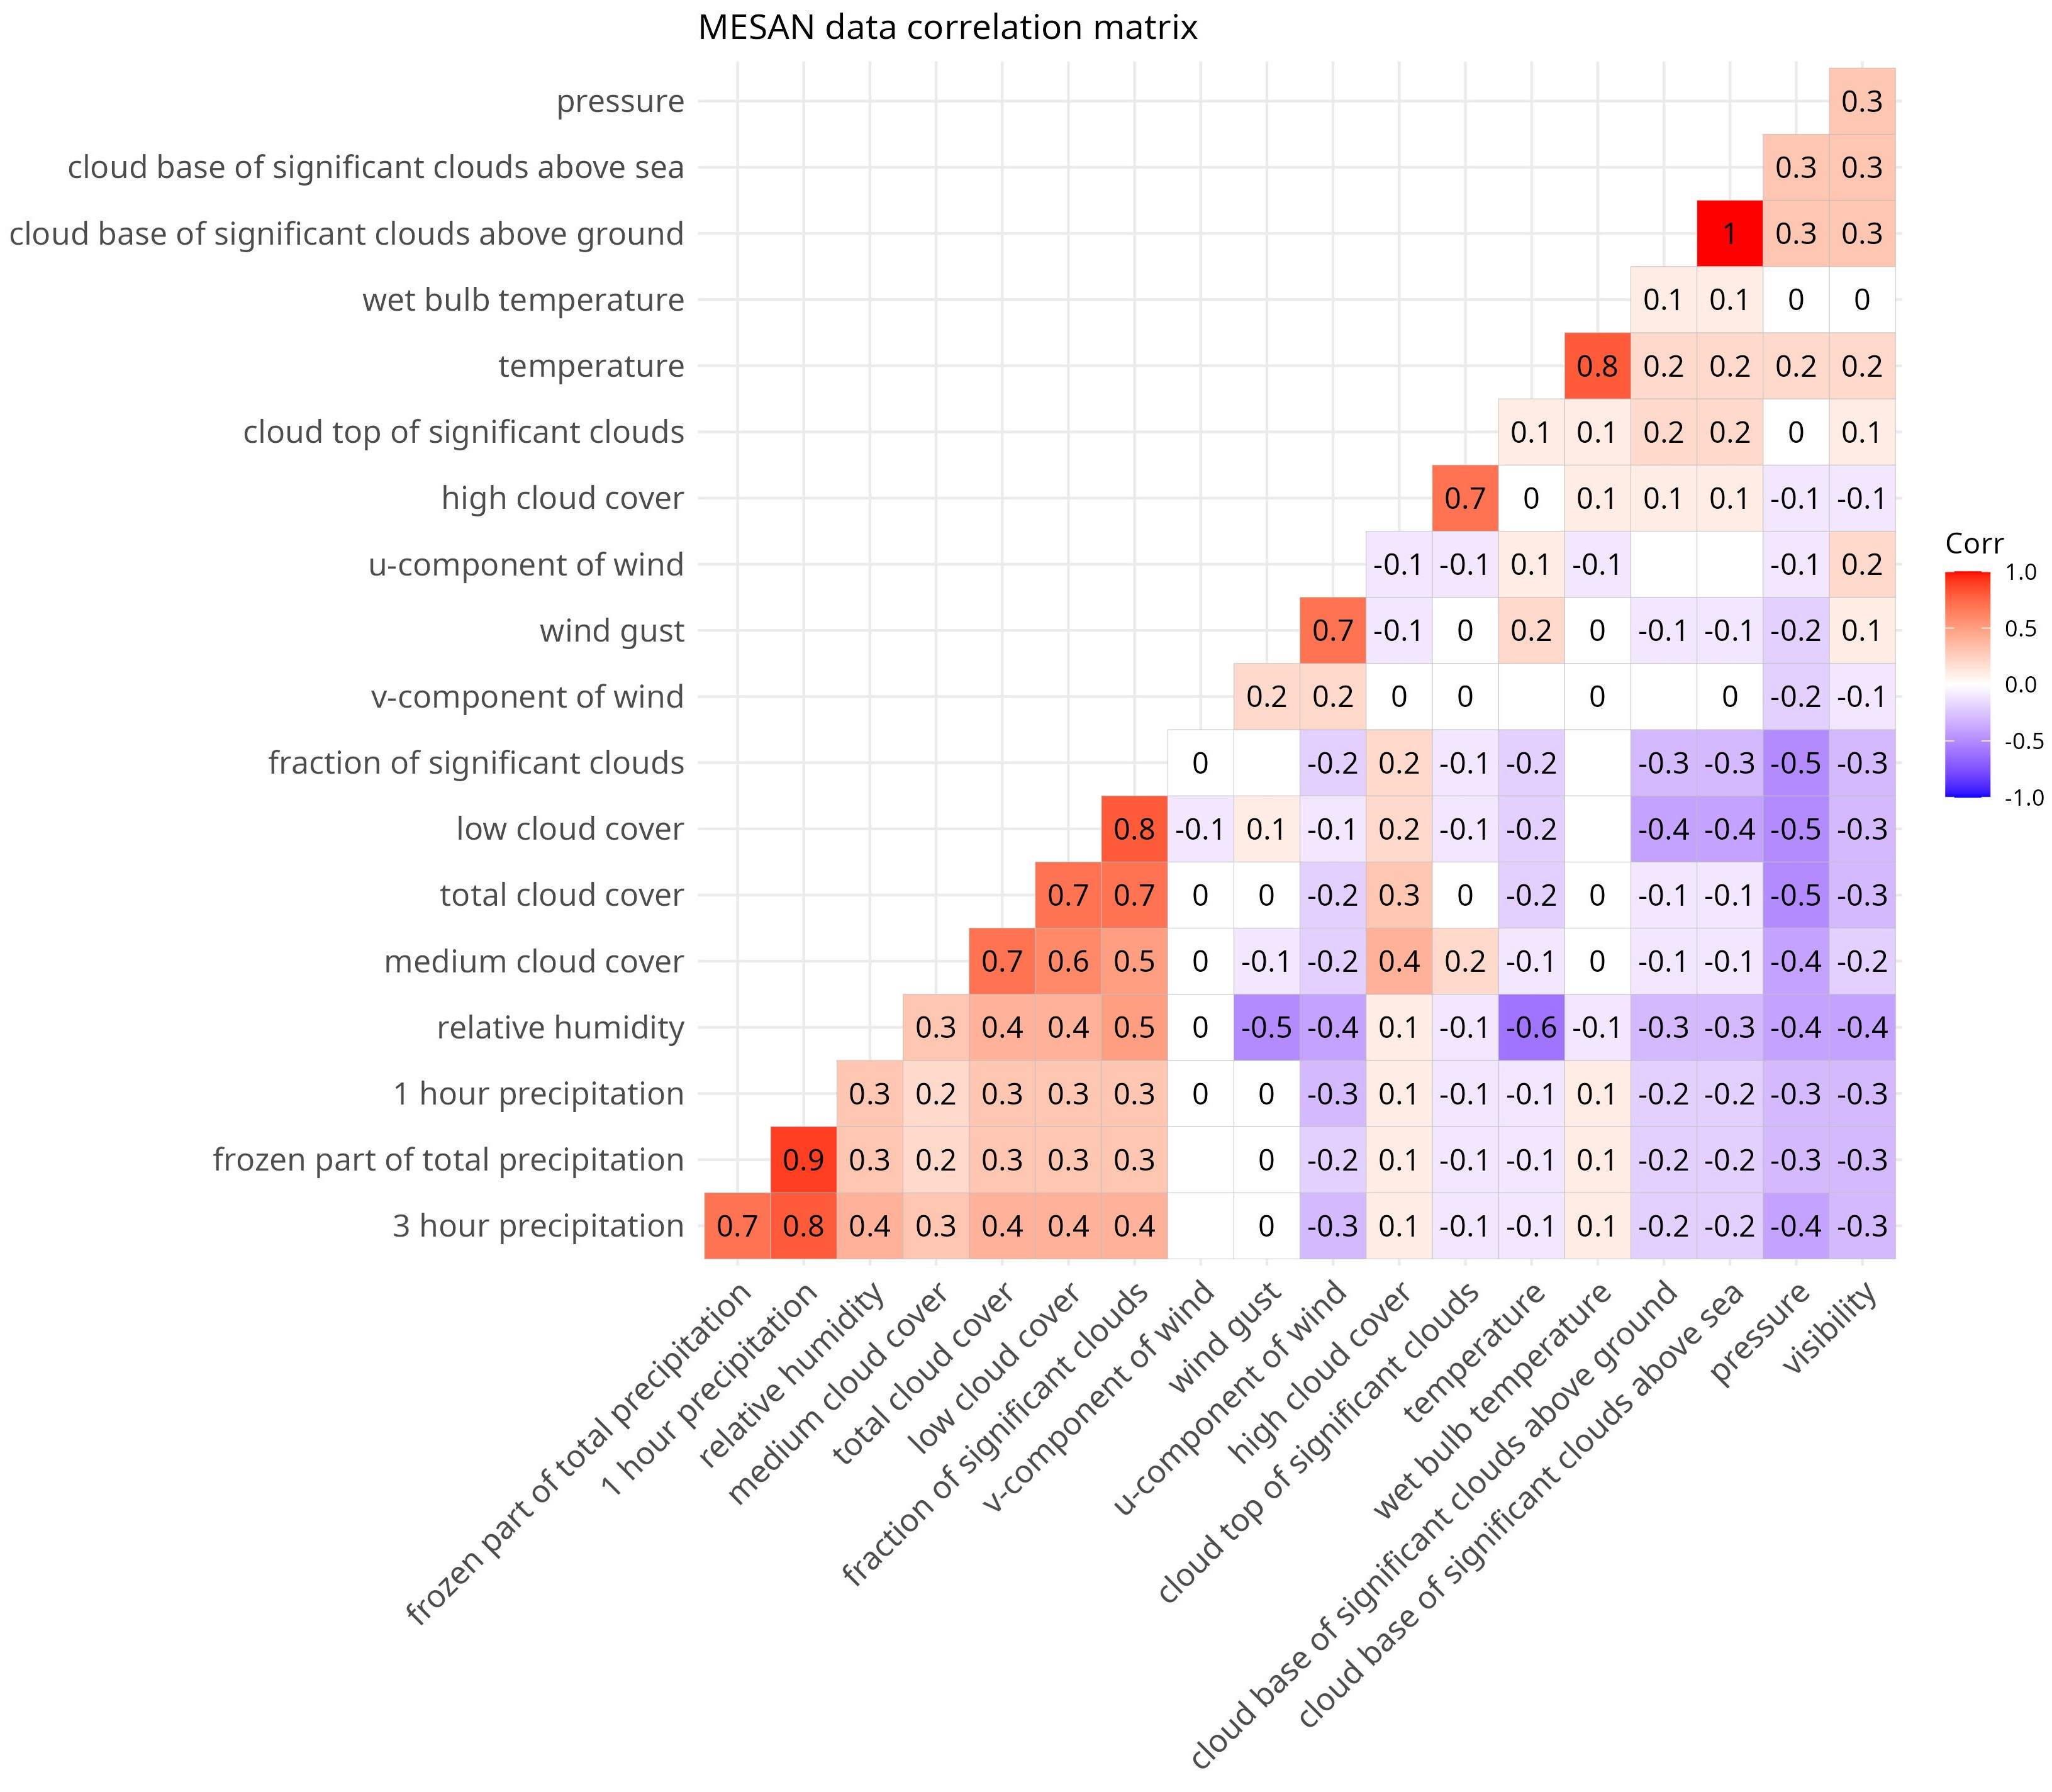
\includegraphics[width=\textwidth, keepaspectratio]{figures/mesan-covariance-matrix-before-analysis}
	\caption{Covariance matrix of the MESAN dataset, before analysis.}
	\label{fig:mesan-covariance-matrix-before-analysis}
\end{figure}

\begin{figure}[H]
	\centering
	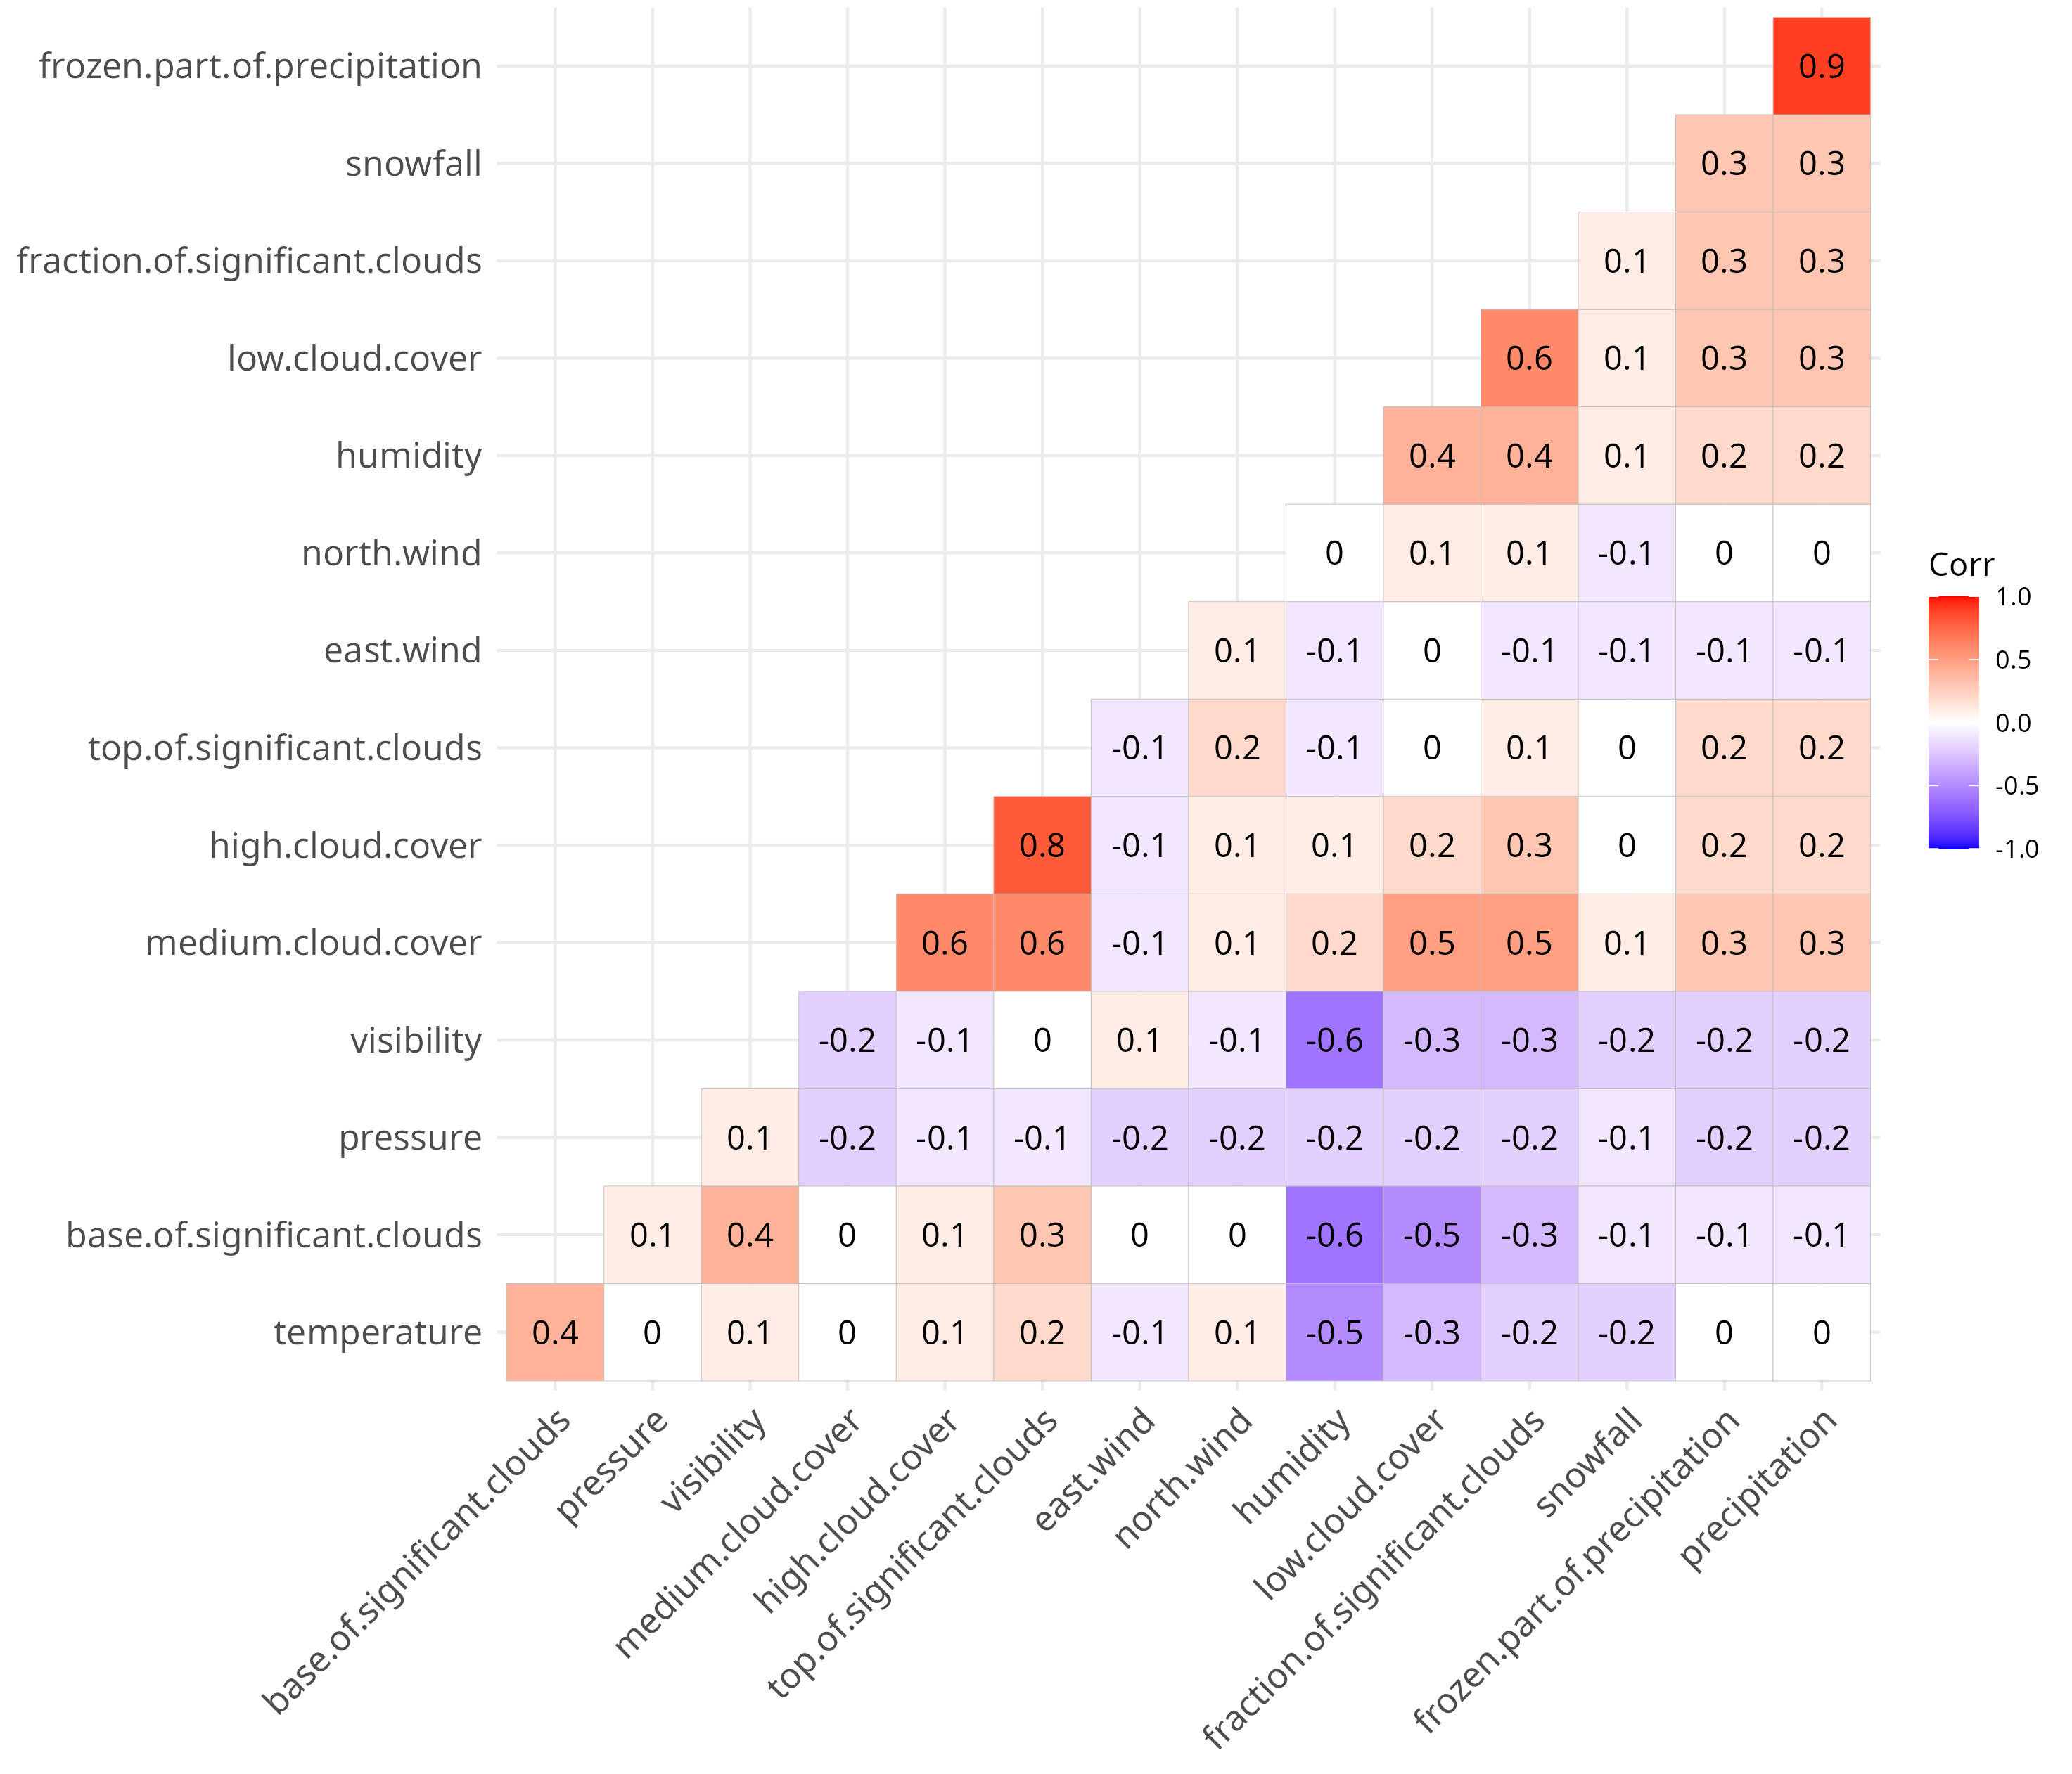
\includegraphics[width=\textwidth, keepaspectratio]{figures/mesan-covariance-matrix-after-analysis}
	\caption{Covariance matrix of the MESAN dataset, after analysis.}
	\label{fig:mesan-covariance-matrix-after-analysis}
\end{figure}

\newpage
The correlation analysis reveals that some parameters have a high correlation coefficient (0.8 or higher), as shown in table \ref{tbl:correlation-high}, while others have a medium correlation coefficient (between 0.6 and 0.8), as shown in table \ref{tbl:correlation-medium}.

\begin{table}[H]
	\centering
	\begin{tabular}{| p{0.4\linewidth} | p{0.4\linewidth} | p{0.2\linewidth} |}
		\hline
		\textbf{Parameter 1} & \textbf{Parameter 2} & \textbf{Correlation} \\
		\hline \hline
		1h precipitation & 3h precipitation & 0.8 \\
		\hline
		1h precipitation & frozen part of total precipitation & 0.9 \\
		\hline
		Low cloud cover & fraction of significant clouds & 0.8 \\
		\hline
		Temperature & wet-bulb temperature & 0.8 \\
		\hline
		Cloud base of significant clouds above ground & cloud base of significant clouds above sea & 1 \\
		\hline
	\end{tabular}
	\caption{Parameter pairs with high correlation (0.8+).}
	\label{tbl:correlation-high}
\end{table}

\begin{table}[H]
	\centering
	\begin{tabular}{|c|c|c|}
		\hline
		\textbf{Parameter 1} & \textbf{Parameter 2} & \textbf{Correlation} \\
		\hline \hline
		3h precipitation & Frozen part of total precipitation & 0.7 \\
		\hline
		Relative humidity & Temperature & -0.6 \\
		\hline
		Medium cloud cover & Total cloud cover & 0.7 \\
		\hline
		Medium cloud cover & Low cloud cover & 0.6 \\
		\hline
		Total cloud cover & Low cloud cover & 0.7 \\
		\hline
		Total cloud cover & Fraction of significant clouds & 0.7 \\
		\hline
		Wind gust & U-component of wind & 0.7 \\
		\hline
		High cloud cover & cloud top of significant clouds & 0.7 \\
		\hline
	\end{tabular}
	\caption{Parameter pairs with medium correlation (between 0.6 and 0.8).}
	\label{tbl:correlation-medium}
\end{table}

\newpage
\subsection{Principle Component Analysis}
\label{sec:analysis-mesan-pca}

Table \ref{tbl:pca} presents a summary of the principal components, while Table \ref{tbl:pcx} provides a detailed analysis of the loadings of the top three principal components, together comprised of over 50\% of the variance in the MESAN dataset. 

\begin{table}[H]
	\centering
	\begin{tabular}{|c|c|c|c|}
		\hline
		\textbf{PC} & \textbf{Standard deviation} & \textbf{Proportion of variance} & \textbf{Cumulative proportion} \\
		\hline \hline
		 1 & 1.92 & 0.25 & 0.25 \\
		\hline
		 2 & 1.56 & 0.16 & 0.40 \\
		\hline
		 3 & 1.18 & 0.09 & 0.50 \\
		\hline
		 4 & 1.13 & 0.09 & 0.59 \\
		\hline
		 5 & 1.02 & 0.07 & 0.66 \\
		\hline
		 6 & 0.96 & 0.06 & 0.72 \\
		\hline
		 7 & 0.92 & 0.06 & 0.77 \\
		\hline
		 8 & 0.85 & 0.05 & 0.82 \\
		\hline
		 9 & 0.81 & 0.04 & 0.87 \\
		\hline
		10 & 0.76 & 0.04 & 0.90 \\
		\hline
		11 & 0.60 & 0.02 & 0.93 \\
		\hline
		12 & 0.59 & 0.02 & 0.95 \\
		\hline
		13 & 0.56 & 0.02 & 0.97 \\
		\hline
		14 & 0.49 & 0.02 & 0.99 \\
		\hline
		15 & 0.43 & 0.01 & 1.00 \\
		\hline
	\end{tabular}
	\caption{Summary of the principle component analysis.}
	\label{tbl:pca}
\end{table}

\begin{table}[H]
	\centering
	\begin{tabular}{|c|c|c|c|}
		\hline
		\textbf{Parameter} & \textbf{PC1} & \textbf{PC2} & \textbf{PC3} \\
		\hline \hline
		pressure                       & -0.21 & -0.02 & -0.02 \\
		\hline
		temperature                    & -0.15 &  0.37 & -0.10 \\
		\hline
		visibility                     & -0.28 &  0.15 &  0.08 \\
		\hline
		east.wind                      & -0.04 & -0.08 &  0.18 \\
		\hline
		north.wind                     &  0.09 &  0.12 &  0.17 \\
		\hline
		humidity                       &  0.32 & -0.28 &  0.07 \\
		\hline
		low.cloud.cover                &  0.39 & -0.15 &  0.21 \\
		\hline
		medium.cloud.cover             &  0.37 &  0.25 &  0.22 \\
		\hline
		high.cloud.cover               &  0.28 &  0.43 &  0.17 \\
		\hline
		fraction.of.significant.clouds &  0.37 & -0.06 &  0.20 \\
		\hline
		base.of.significant.clouds     & -0.21 &  0.43 & -0.05 \\
		\hline
		top.of.significant.clouds      &  0.17 &  0.51 &  0.11 \\
		\hline
		frozen.part.of.precipitation   &  0.30 &  0.08 & -0.55 \\
		\hline
		precipitation                  &  0.25 &  0.09 & -0.56 \\
		\hline
		snowfall                       &  0.13 & -0.04 & -0.35 \\
		\hline
	\end{tabular}
	\caption{Loading of the first three PCs, together representing over 50\% of the variation of the dataset.}
	\label{tbl:pcx}
\end{table}

\newpage
\section{Hyperparameter Tuning}
\label{sec:analysis-hyperparameters}

The following list shows the resulting hyperparameters derived by the genetic algorithm (refer to section \ref{sec:method-hypertuning} on page \pageref{sec:method-hypertuning}):

\begin{itemize}
	\item Batch size: 128
	\item Optimizer: Adam
	\item Activation function for the recurrent layers: tanh
	\item Activation function for the dense layers: relu
	\item Dropout for the recurrent layers: 0.2
	\item Dropout for the dense layers: 0.2
	\item Number of recurrent layers: 2
	\item Number of dense layers: 0
	\item Number of units in the recurrent layers: 256
	\item Number of units in the dense layers: 64
	\item Normalization between recurrent layers: True
	\item Normalization between dense layers: True
\end{itemize}

It is important to note that these hyperparameters might not be the most efficient in every scenario, and will likely have to be re-evaluated after making changes in the dataset or regarding model type and lookback/lookahead combination.

\section{Model Evaluation}

Table \ref{tbl:dense}, \ref{tbl:rnn}, \ref{tbl:lstm} and \ref{tbl:gru} presents the metrics gathered from the evaluation of DNN, SRNN, LSTM and GRU models respectively. All models were trained over eight epochs using the stratified 10-fold cross validation method. As such, each metric is an average over ten iterations, where the original dataset is split into ten parts, eight parts used for training, one for validation and one for testing in each fold.

Each table row shows the parameters lookback, lookahead, training time (TT), accuracy (AC), F1-Score (F1), Mean Absolute Error (ME) and Wilson Score (WS) measured from both the training and testing phases of each model. Lookback and lookahead are specified in hours, training time in seconds and the remaining four metrics as percentages. As the feature sequence have to be randomly shifted for every lookahead value, some combinations of lookback and lookahead (e.g. 72 and 3) exceeds the available time points, and the metrics are labeled as missing (NA). As the dense model is unable to consider timeseries (see \ref{sec:model-selection-dnn} on page \pageref{sec:model-selection-dnn}), the only lookback available is \texttt{1}.

\newpage
\begin{table}[H]
	\centering
	\begin{tabular}{|c|c||c|c|c|c|c|}
		\hline
		\textbf{Lookback} & \textbf{Lookahead} & \textbf{TT} & \textbf{AC} & \textbf{F1} & \textbf{ME} & \textbf{WS} \\
		\hline \hline
		 1 &  1 & 8.77 & 88.57 & 89.08 & 14.83 & 12.27 \\
		\hline
		 1 &  3 & 8.80 & 88.84 & 89.37 & 14.61 & 12.00 \\
		\hline
		 1 &  6 & 8.75 & 88.98 & 89.57 & 14.37 & 11.85 \\
		\hline
		 1 & 12 & 8.79 & 89.00 & 89.75 & 14.44 & 11.83 \\
		\hline
		 1 & 24 & 8.79 & 88.85 & 89.86 & 14.54 & 11.99 \\
		%\hline
		 %3 &  1 & 8.79 & 88.58 & 89.09 & 14.84 & 12.26 \\
		%\hline
		 %%3 &  3 & 8.78 & 88.81 & 89.37 & 14.54 & 12.03 \\
		%\hline
		 %3 &  6 & 8.77 & 89.04 & 89.64 & 14.40 & 11.79 \\
		%\hline
		 %3 & 12 & 8.80 & 89.06 & 89.78 & 14.27 & 11.77 \\
		%\hline
		 %3 & 24 & 8.77 & 88.89 & 89.92 & 14.45 & 11.94 \\
		%\hline
		 %6 &  1 & 8.79 & 88.53 & 89.04 & 14.79 & 12.32 \\
		%\hline
		 %6 &  3 & 8.74 & 88.76 & 89.28 & 14.63 & 12.07 \\
		%\hline
		 %6 &  6 & 8.77 & 89.01 & 89.61 & 14.36 & 11.82 \\
		%\hline
		 %6 & 12 & 8.73 & 88.94 & 89.72 & 14.54 & 11.89 \\
		%\hline
		 %6 & 24 & 8.76 & 88.71 & 89.75 & 14.62 & 12.13 \\
		%\hline
		%12 &  1 & 8.76 & 88.57 & 89.08 & 14.81 & 12.27 \\
		%\hline
		%12 &  3 & 8.78 & 88.83 & 89.37 & 14.61 & 12.01 \\
		%\hline
		%12 &  6 & 8.77 & 88.98 & 89.59 & 14.32 & 11.85 \\
		%\hline
		%12 & 12 & 8.72 & 88.89 & 89.65 & 14.51 & 11.94 \\
		%\hline
		%12 & 24 & 8.77 & 88.69 & 89.75 & 14.58 & 12.14 \\
		%\hline
		%24 &  1 & 8.76 & 88.56 & 89.06 & 14.78 & 12.29 \\
		%\hline
		%24 &  3 & 8.73 & 88.76 & 89.30 & 14.59 & 12.08 \\
		%\hline
		%24 &  6 & 8.77 & 88.99 & 89.60 & 14.39 & 11.84 \\
		%\hline
		%24 & 12 & 8.75 & 88.99 & 89.71 & 14.29 & 11.84 \\
		%\hline
		%24 & 24 & 8.78 & 88.84 & 89.86 & 14.52 & 12.00 \\
		%\hline
		%48 &  1 & 8.76 & 88.61 & 89.12 & 14.85 & 12.23 \\
		%\hline
		%48 &  3 & 8.74 & 88.84 & 89.39 & 14.51 & 11.99 \\
		%\hline
		%48 &  6 & 8.72 & 89.04 & 89.64 & 14.39 & 11.79 \\
		%\hline
		%48 & 12 & 8.75 & 89.01 & 89.77 & 14.41 & 11.82 \\
		%\hline
		%48 & 24 & 8.75 & 88.67 & 89.73 & 14.69 & 12.17 \\
		%\hline
		%72 &  1 & 8.75 & 88.66 & 89.16 & 14.78 & 12.18 \\
		%\hline
		%72 &  3 &   NA &    NA &    NA &    NA &    NA \\
		%\hline
		%72 &  6 &   NA &    NA &    NA &    NA &    NA \\
		%\hline
		%72 & 12 &   NA &    NA &    NA &    NA &    NA \\
		%\hline
		%72 & 24 &   NA &    NA &    NA &    NA &    NA \\
		\hline
	\end{tabular}
	\caption{Metrics from model: DENSE}
	\label{tbl:dense}
\end{table}

\newpage
\begin{table}[H]
	\centering
	\begin{tabular}{|c|c||c|c|c|c|c|}
		\hline
		\textbf{Lookback} & \textbf{Lookahead} & \textbf{TT} & \textbf{AC} & \textbf{F1} & \textbf{ME} & \textbf{WS} \\
		\hline \hline
		 1 &  1 & 132.04 & 89.33 & 89.77 & 13.79 & 11.49 \\
		\hline
		 1 &  3 & 130.83 & 89.37 & 89.91 & 13.72 & 11.45 \\
		\hline
		 1 &  6 & 130.02 & 89.60 & 90.14 & 13.46 & 11.21 \\
		\hline
		 1 & 12 & 130.85 & 89.19 & 89.93 & 13.96 & 11.63 \\
		\hline
		 1 & 24 & 131.12 & 88.73 & 89.84 & 14.24 & 12.11 \\
		\hline
		 3 &  1 & 130.19 & 89.14 & 89.62 & 14.01 & 11.68 \\
		\hline
		 3 &  3 & 129.05 & 89.08 & 89.46 & 14.67 & 11.74 \\
		\hline
		 3 &  6 & 129.22 & 89.54 & 90.09 & 13.53 & 11.28 \\
		\hline
		 3 & 12 & 130.54 & 89.49 & 90.17 & 13.66 & 11.33 \\
		\hline
		 3 & 24 & 130.01 & 89.36 & 90.31 & 13.72 & 11.46 \\
		\hline
		 6 &  1 & 130.29 & 89.18 & 89.66 & 14.03 & 11.64 \\
		\hline
		 6 &  3 & 130.78 & 89.32 & 89.81 & 13.70 & 11.50 \\
		\hline
		 6 &  6 & 130.64 & 89.00 & 89.57 & 14.05 & 11.83 \\
		\hline
		 6 & 12 & 131.10 & 89.57 & 90.27 & 13.58 & 11.24 \\
		\hline
		 6 & 24 & 130.55 & 89.46 & 90.45 & 13.69 & 11.36 \\
		\hline
		12 &  1 & 129.52 & 88.78 & 89.26 & 14.60 & 12.06 \\
		\hline
		12 &  3 & 131.15 & 88.81 & 89.33 & 14.41 & 12.03 \\
		\hline
		12 &  6 & 128.89 & 89.54 & 90.09 & 13.46 & 11.27 \\
		\hline
		12 & 12 & 130.35 & 89.71 & 90.43 & 13.32 & 11.10 \\
		\hline
		12 & 24 & 129.01 & 88.98 & 89.93 & 14.41 & 11.85 \\
		\hline
		24 &  1 & 129.58 & 88.57 & 89.13 & 14.62 & 12.27 \\
		\hline
		24 &  3 & 130.07 & 89.33 & 89.83 & 13.69 & 11.49 \\
		\hline
		24 &  6 & 129.76 & 89.71 & 90.16 & 13.53 & 11.10 \\
		\hline
		24 & 12 & 131.16 & 89.23 & 89.91 & 14.22 & 11.59 \\
		\hline
		24 & 24 & 129.80 & 89.24 & 90.16 & 13.70 & 11.58 \\
		\hline
		48 &  1 & 128.39 & 89.39 & 89.84 & 13.77 & 11.43 \\
		\hline
		48 &  3 & 129.28 & 89.35 & 89.81 & 13.84 & 11.47 \\
		\hline
		48 &  6 & 128.58 & 89.28 & 89.82 & 14.04 & 11.54 \\
		\hline
		48 & 12 & 129.65 & 89.36 & 90.11 & 13.84 & 11.46 \\
		\hline
		48 & 24 & 129.65 & 88.76 & 89.85 & 14.53 & 12.08 \\
		\hline
		72 &  1 & 130.95 & 89.15 & 89.61 & 14.12 & 11.67 \\
		\hline
		72 &  3 &     NA &    NA &    NA &    NA &    NA \\
		\hline
		72 &  6 &     NA &    NA &    NA &    NA &    NA \\
		\hline
		72 & 12 &     NA &    NA &    NA &    NA &    NA \\
		\hline
		72 & 24 &     NA &    NA &    NA &    NA &    NA \\
		\hline
	\end{tabular}
	\caption{Metrics from model: Simple RNN}
	\label{tbl:rnn}
\end{table}

\newpage
\begin{table}[H]
	\centering
	\begin{tabular}{|c|c||c|c|c|c|c|}
		\hline
		\textbf{Lookback} & \textbf{Lookahead} & \textbf{TT} & \textbf{AC} & \textbf{F1} & \textbf{ME} & \textbf{WS} \\
		\hline \hline
		 1 &  1 & 57.92 & 91.77 & 92.05 & 10.37 &  8.96 \\
		\hline
		 1 &  3 & 57.76 & 91.96 & 92.25 & 10.09 &  8.76 \\
		\hline
		 1 &  6 & 57.66 & 91.42 & 91.69 & 10.93 &  9.32 \\
		\hline
		 1 & 12 & 57.56 & 87.93 & 87.94 & 16.02 & 12.93 \\
		\hline
		 1 & 24 & 57.36 & 85.09 & 85.01 & 19.93 & 15.85 \\
		\hline
		 3 &  1 & 57.59 & 79.25 & 29.77 & 24.36 & 21.83 \\
		\hline
		 3 &  3 & 57.45 & 81.06 & 38.78 & 23.83 & 19.98 \\
		\hline
		 3 &  6 & 57.56 & 80.86 & 47.96 & 24.85 & 20.19 \\
		\hline
		 3 & 12 & 57.54 & 80.82 & 58.46 & 24.29 & 20.23 \\
		\hline
		 3 & 24 & 57.40 & 80.09 & 66.76 & 25.39 & 20.97 \\
		\hline
		 6 &  1 & 57.62 & 79.83 & 22.31 & 24.06 & 21.24 \\
		\hline
		 6 &  3 & 57.68 & 81.37 & 30.83 & 22.95 & 19.67 \\
		\hline
		 6 &  6 & 57.54 & 81.39 & 37.86 & 22.77 & 19.65 \\
		\hline
		 6 & 12 & 57.46 & 81.52 & 48.71 & 23.81 & 19.51 \\
		\hline
		 6 & 24 & 57.39 & 82.21 & 60.31 & 23.83 & 18.81 \\
		\hline
		12 &  1 & 57.65 & 81.07 & 19.56 & 25.31 & 19.97 \\
		\hline
		12 &  3 & 57.65 & 83.54 & 26.70 & 23.51 & 17.45 \\
		\hline
		12 &  6 & 57.62 & 81.66 & 33.38 & 24.57 & 19.37 \\
		\hline
		12 & 12 & 57.62 & 79.83 & 43.01 & 25.73 & 21.24 \\
		\hline
		12 & 24 & 57.54 & 77.86 & 53.83 & 27.49 & 23.24 \\
		\hline
		24 &  1 & 57.62 & 77.53 & 17.36 & 27.76 & 23.58 \\
		\hline
		24 &  3 & 57.57 & 80.35 & 24.17 & 25.78 & 20.71 \\
		\hline
		24 &  6 & 57.44 & 78.96 & 29.66 & 27.04 & 22.12 \\
		\hline
		24 & 12 & 57.51 & 81.93 & 40.14 & 25.21 & 19.10 \\
		\hline
		24 & 24 & 57.43 & 75.02 & 49.11 & 29.05 & 26.13 \\
		\hline
		48 &  1 & 57.68 & 70.53 & 12.59 & 31.48 & 30.69 \\
		\hline
		48 &  3 & 57.59 & 69.44 & 17.71 & 33.07 & 31.79 \\
		\hline
		48 &  6 & 57.58 & 73.47 & 24.20 & 30.68 & 27.71 \\
		\hline
		48 & 12 & 57.49 & 75.90 & 34.89 & 29.41 & 25.24 \\
		\hline
		48 & 24 & 57.51 & 79.12 & 46.83 & 27.14 & 21.96 \\
		\hline
		72 &  1 & 57.69 & 85.46 & 11.07 & 27.43 & 15.47 \\
		\hline
		72 &  3 &    NA &    NA &    NA &    NA &    NA \\
		\hline
		72 &  6 &    NA &    NA &    NA &    NA &    NA \\
		\hline
		72 & 12 &    NA &    NA &    NA &    NA &    NA \\
		\hline
		72 & 24 &    NA &    NA &    NA &    NA &    NA \\
		\hline
	\end{tabular}
	\caption{Metrics from model: LSTM}
	\label{tbl:lstm}
\end{table}

\newpage
\begin{table}[H]
	\centering
	\begin{tabular}{|c|c||c|c|c|c|c|}
		\hline
		\textbf{Lookback} & \textbf{Lookahead} & \textbf{TT} & \textbf{AC} & \textbf{F1} & \textbf{ME} & \textbf{WS} \\
		\hline \hline
		 1 &  1 & 48.67 & 91.94 & 92.20 &  9.73 &  8.78 \\
		\hline
		 1 &  3 & 48.51 & 92.19 & 92.47 &  9.45 &  8.52 \\
		\hline
		 1 &  6 & 48.42 & 91.60 & 91.87 & 10.36 &  9.14 \\
		\hline
		 1 & 12 & 48.46 & 88.24 & 88.24 & 15.34 & 12.61 \\
		\hline
		 1 & 24 & 48.22 & 85.26 & 85.03 & 19.19 & 15.68 \\
		\hline
		 3 &  1 & 48.53 & 80.75 & 31.06 & 23.11 & 20.30 \\
		\hline
		 3 &  3 & 48.45 & 81.90 & 39.71 & 23.15 & 19.13 \\
		\hline
		 3 &  6 & 48.40 & 82.07 & 48.82 & 23.18 & 18.95 \\
		\hline
		 3 & 12 & 48.29 & 81.16 & 59.21 & 23.76 & 19.87 \\
		\hline
		 3 & 24 & 48.25 & 79.99 & 66.83 & 24.34 & 21.07 \\
		\hline
		 6 &  1 & 48.37 & 80.81 & 23.56 & 22.64 & 20.24 \\
		\hline
		 6 &  3 & 48.42 & 83.27 & 32.52 & 20.89 & 17.73 \\
		\hline
		 6 &  6 & 48.34 & 81.88 & 39.46 & 21.36 & 19.14 \\
		\hline
		 6 & 12 & 48.32 & 82.73 & 50.62 & 21.46 & 18.27 \\
		\hline
		 6 & 24 & 48.19 & 83.11 & 62.34 & 21.97 & 17.89 \\
		\hline
		12 &  1 & 48.42 & 82.74 & 23.04 & 21.29 & 18.27 \\
		\hline
		12 &  3 & 48.38 & 83.50 & 30.65 & 20.65 & 17.48 \\
		\hline
		12 &  6 & 48.35 & 83.09 & 37.26 & 21.35 & 17.91 \\
		\hline
		12 & 12 & 48.32 & 81.34 & 47.03 & 23.42 & 19.69 \\
		\hline
		12 & 24 & 48.07 & 80.11 & 57.42 & 24.31 & 20.95 \\
		\hline
		24 &  1 & 48.24 & 82.18 & 19.98 & 23.20 & 18.84 \\
		\hline
		24 &  3 & 48.37 & 79.52 & 24.41 & 25.90 & 21.55 \\
		\hline
		24 &  6 & 48.30 & 81.71 & 32.17 & 23.94 & 19.32 \\
		\hline
		24 & 12 & 48.18 & 82.46 & 43.36 & 22.99 & 18.55 \\
		\hline
		24 & 24 & 48.19 & 79.07 & 53.86 & 25.27 & 22.01 \\
		\hline
		48 &  1 & 48.39 & 72.47 & 14.02 & 29.93 & 28.72 \\
		\hline
		48 &  3 & 48.45 & 72.74 & 19.61 & 30.28 & 28.45 \\
		\hline
		48 &  6 & 48.29 & 75.95 & 26.60 & 27.97 & 25.19 \\
		\hline
		48 & 12 & 48.26 & 79.12 & 38.82 & 26.09 & 21.96 \\
		\hline
		48 & 24 & 48.10 & 81.33 & 51.76 & 23.78 & 19.70 \\
		\hline
		72 &  1 & 48.36 & 82.63 & 14.92 & 24.52 & 18.38 \\
		\hline
		72 &  3 &    NA &    NA &    NA &    NA &    NA \\
		\hline
		72 &  6 &    NA &    NA &    NA &    NA &    NA \\
		\hline
		72 & 12 &    NA &    NA &    NA &    NA &    NA \\
		\hline
		72 & 24 &    NA &    NA &    NA &    NA &    NA \\
		\hline
	\end{tabular}
	\caption{Metrics from model: GRU}
	\label{tbl:gru}
\end{table}

%train_lstm <- c(57.92 57.76, 57.66, 57.56, 57.36, 57.59, 57.45, 57.56, 57.54, 57.40, 57.62, 57.68, 57.54, 57.46, 57.39, 57.65, 57.65, 57.62, 57.62, 57.54, 57.62, 57.57, 57.44, 57.51, 57.43, 57.68, 57.59, 57.58, 57.49, 57.51, 57.69)
%a_lstm <- c(91.77 , 91.96 , 91.42 , 87.93 , 85.09 , 79.25 , 81.06 , 80.86 , 80.82 , 80.09 , 79.83 , 81.37 , 81.39 , 81.52 , 82.21 , 81.07, 83.54, 81.66, 79.83, 77.86, 77.53, 80.35, 78.96, 81.93, 75.02, 70.53, 69.44, 73.47, 75.90, 79.12, 85.46)
%f_lstm <- c(92.05 , 92.25 , 91.69 , 87.94 , 85.01 , 29.77 , 38.78 , 47.96 , 58.46 , 66.76 , 22.31 , 30.83 , 37.86 , 48.71 , 60.31 , 19.56, 26.70, 33.38, 43.01, 53.83, 17.36, 24.17, 29.66, 40.14, 49.11, 12.59, 17.71, 24.20, 34.89, 46.83, 11.07)
%mae_lstm <- c(10.37 , 10.09 , 10.93 , 16.02 , 19.93 , 24.36 , 23.83 , 24.85 , 24.29 , 25.39 , 24.06 , 22.95 , 22.77 , 23.81 , 23.83 , 25.31, 23.51, 24.57, 25.73, 27.49, 27.76, 25.78, 27.04, 25.21, 29.05, 31.48, 33.07, 30.68, 29.41, 27.14, 27.43)
%train_gru <- c(48.67, 48.51, 48.42, 48.46, 48.22, 48.53, 48.45, 48.40, 48.29, 48.25, 48.37, 48.42, 48.34, 48.32, 48.19, 48.42, 48.38, 48.35, 48.32, 48.07, 48.24, 48.37, 48.30, 48.18, 48.19, 48.39, 48.45, 48.29, 48.26, 48.10, 48.36)
%a_gru <- c(91.94, 92.19, 91.60, 88.24, 85.26, 80.75, 81.90, 82.07, 81.16, 79.99, 80.81, 83.27, 81.88, 82.73, 83.11, 82.74, 83.50, 83.09, 81.34, 80.11, 82.18, 79.52, 81.71, 82.46, 79.07, 72.47, 72.74, 75.95, 79.12, 81.33, 82.63)
%f_gru <- c(92.20, 92.47, 91.87, 88.24, 85.03, 31.06, 39.71, 48.82, 59.21, 66.83, 23.56, 32.52, 39.46, 50.62, 62.34, 23.04, 30.65, 37.26, 47.03, 57.42, 19.98, 24.41, 32.17, 43.36, 53.86, 14.02, 19.61, 26.60, 38.82, 51.76, 14.92)
%mae_gru <- c(9.73, 9.45, 10.36, 15.34, 19.19, 23.11, 23.15, 23.18, 23.76, 24.34, 22.64, 20.89, 21.36, 21.46, 21.97, 21.29, 20.65, 21.35, 23.42, 24.31, 23.20, 25.90, 23.94, 22.99, 25.27, 29.93, 30.28, 27.97, 26.09, 23.78, 24.52)
%train_dense <- c(8.77, 8.80, 8.75, 8.79, 8.79, 8.79, 8.78, 8.77, 8.80, 8.77, 8.79, 8.74, 8.77, 8.73, 8.76, 8.76, 8.78, 8.77, 8.72, 8.77, 8.76, 8.73, 8.77, 8.75, 8.78, 8.76, 8.74, 8.72, 8.75, 8.75, 8.75)
%a_dense <- c(88.57 , 88.84 , 88.98 , 89.00 , 88.85 , 88.58 , 88.81 , 89.04 , 89.06 , 88.89 , 88.53 , 88.76 , 89.01 , 88.94 , 88.71 , 88.57 , 88.83 , 88.98 , 88.89 , 88.69 , 88.56 , 88.76 , 88.99 , 88.99 , 88.84 , 88.61 , 88.84 , 89.04 , 89.01 , 88.67 , 88.66)
%f_dense <- c(89.08 , 89.37 , 89.57 , 89.75 , 89.86 , 89.09 , 89.37 , 89.64 , 89.78 , 89.92 , 89.04 , 89.28 , 89.61 , 89.72 , 89.75 , 89.08 , 89.37 , 89.59 , 89.65 , 89.75 , 89.06 , 89.30 , 89.60 , 89.71 , 89.86 , 89.12 , 89.39 , 89.64 , 89.77 , 89.73 , 89.16)
%mae_dense <- c(14.83 , 14.61 , 14.37 , 14.44 , 14.54 , 14.84 , 14.54 , 14.40 , 14.27 , 14.45 , 14.79 , 14.63 , 14.36 , 14.54 , 14.62 , 14.81 , 14.61 , 14.32 , 14.51 , 14.58 , 14.78 , 14.59 , 14.39 , 14.29 , 14.52 , 14.85 , 14.51 , 14.39 , 14.41 , 14.69 , 14.78)
%c_dense <- c(12.27, 12.00, 11.85, 11.83, 11.99, 12.26, 12.03, 11.79, 11.77, 11.94, 12.32, 12.07, 11.82, 11.89, 12.13, 12.27, 12.01, 11.85, 11.94, 12.14, 12.29, 12.08, 11.84, 11.84, 12.00, 12.23, 11.99, 11.79, 11.82, 12.17, 12.18)
%train_srnn <- c(132.04 , 130.83 , 130.02 , 130.85 , 131.12 , 130.19 , 129.05 , 129.22 , 130.54 , 130.01 , 130.29 , 130.78 , 130.64 , 131.10 , 130.55 , 129.52 , 131.15 , 128.89 , 130.35 , 129.01 , 129.58 , 130.07 , 129.76 , 131.16 , 129.80 , 128.39 , 129.28 , 128.58 , 129.65 , 129.65 , 130.95)
%a_srnn <- c(89.33 , 89.37 , 89.60 , 89.19 , 88.73 , 89.14 , 89.08 , 89.54 , 89.49 , 89.36 , 89.18 , 89.32 , 89.00 , 89.57 , 89.46 , 88.78 , 88.81 , 89.54 , 89.71 , 88.98 , 88.57 , 89.33 , 89.71 , 89.23 , 89.24 , 89.39 , 89.35 , 89.28 , 89.36 , 88.76 , 89.15)
%f_srnn <- c(89.77 , 89.91 , 90.14 , 89.93 , 89.84 , 89.62 , 89.46 , 90.09 , 90.17 , 90.31 , 89.66 , 89.81 , 89.57 , 90.27 , 90.45 , 89.26 , 89.33 , 90.09 , 90.43 , 89.93 , 89.13 , 89.83 , 90.16 , 89.91 , 90.16 , 89.84 , 89.81 , 89.82 , 90.11 , 89.85 , 89.61)
%mae_srnn <- c(13.79 , 13.72 , 13.46 , 13.96 , 14.24 , 14.01 , 14.67 , 13.53 , 13.66 , 13.72 , 14.03 , 13.70 , 14.05 , 13.58 , 13.69 , 14.60 , 14.41 , 13.46 , 13.32 , 14.41 , 14.62 , 13.69 , 13.53 , 14.22 , 13.70 , 13.77 , 13.84 , 14.04 , 13.84 , 14.53 , 14.12)
%c_srnn <- c(11.49, 11.45, 11.21, 11.63, 12.11, 11.68, 11.74, 11.28, 11.33, 11.46, 11.64, 11.50, 11.83, 11.24, 11.36, 12.06, 12.03, 11.27, 11.10, 11.85, 12.27, 11.49, 11.10, 11.59, 11.58, 11.43, 11.47, 11.54, 11.46, 12.08, 11.67)

% DENSE:
% - Mean TT: 8.76
% - Mean AC: 88.82
% - Mean F1: 89.50
% - Mean ME: 14.56
% - Mean CF: 12.01

% SRNN:
% - Mean TT: 130.01
% - Mean AC: 89.24
% - Mean F1: 89.88
% - Mean ME: 13.93
% - Mean CF: 11.58

% LSTM:
% - Mean TT: 57.57
% - Mean AC: 80.91
% - Mean F1: 44.35
% - Mean ME: 24.13

% GRU:
% - Mean TT: 48.34
% - Mean AC: 82.16
% - Mean F1: 46.41
% - Mean ME: 22.10

\newpage
The training time appears to be consistent across different combinations of lookback and lookahead values, while varying across models with the SRNN being the slowest by a significant margin. The LSTM and GRU demonstrates similar training times, with GRU being slightly more performant. The DNN model is the fastest by a large margin.

For the DNN and SRNN model, the accuracy and F1 score is very consistent, and does not exhibit much variation with respect to lookback and lookahead. This applies to the confidence of the model as well.

The accuracy and F1 score values for the LSTM and GRU models vary greatly depending on the lookback and lookahead values. Generally, higher lookback values (e.g. 24 and 48) result in lower accuracy and F1 score values, while lower lookback values (e.g. 1 and 3) result in higher accuracy and F1 score values. This might indicate that considering a smaller number of previous time steps for prediction leads to better performance. Increasing the lookahead from 1 to 3 or 6 improves the accuracy and F1 score slightly, but the mean error also increases. This suggests that the model struggles to accurately predict lightning strikes further into the future.

The Mean Absolute Error and Wilson Score for the LSTM and GRU models values also follow a similar trend as accuracy and F1 score. Smaller lookback values result in lower mean absolute error, indicating better prediction accuracy. Increasing the lookahead seems to decrease the confidence of the model, but does not have as drastic effect as lookback.

